The searches for charged \textbf{lepton flavour violation (LFV)}   probe new physics in a manner that is complementary
to the collider, dark
matter, dark energy, and neutrino physics programmes.
They already test NP flavour scales up to  $10^4$~TeV (see Fig.~\ref{fig:NPscales}, light blue), while the sensitivity is expected to substantially increase in the mid-term, 
as shown in Figs.~\ref{fig:cLFV:muon:chrono} 
and~\ref{fig:NPscales} (dark blue). 
The highest sensitivity relies on the use of high-intensity muon beams to search for the ``golden'' $\mu \to e$ transitions~\cite{Baldini:2018uhj}. 

The {\bf short-term} prospects for the different muon channels include:  

\textbf{The ${\mu^+ \to e^+ \gamma}$ decay}: MEG II at PSI~\cite{Baldini:2018nnn}. The signature consists of a back-to-back
photon--positron pair coincident in time,
each with an energy of $m_\mu/2$.
To fully profit from the high intensity $\pi$E5
muon beam ($\sim 10^8$ stopped $\mu^+/$s), 
MEG II detector must succeed in mitigating 
the dominant 
accidental backgrounds. 
For the upgraded detector the 
improvements of resolutions  by roughly a factor 2 should allow 
a factor of ten improvement in the expected sensitivity at the end of the 2020-2023 physics run, giving the projected reach of
BR$(\mu \to e \gamma)< 6 \times 10^{-14}$~\cite{Baldini:2018nnn}. 

\textbf{The ${\mu^+ \to e^+ e^- e^+}$ decay}: Mu3e at PSI~\cite{Blondel:2013ia}.  
The experimental signature 
consists of three time-coincident charged particle tracks from a common
vertex, with the energy of the final state particles 
ranging from below 1~MeV up to $\sim m_\mu/2$.
Excellent timing and vertex resolutions can suppress the dominant
accidental backgrounds, while a very good
resolution of the final state energy successfully controls the intrinsic backgrounds.
In principle,
the sensitivity of Mu3e Phase-I is only limited by the maximal muon rate.
Commissioning is scheduled for 2021, and 
after 3 years of operation
Mu3e Phase-I aims at a sensitivity of $2\times 10^{-15}$ (90\% C.L.)
using the existing $\pi$E5 beamline at PSI~\cite{Blondel:2013ia}.

\textbf{The ${\mu^- - e^-}$ conversion in Al}: 
the neutrinoless conversion process $\mu^- \text{N} \to e^- \text{N}$ has a clean
experimental signature: an outgoing electron with an
energy near the muon mass. 
In the short term, two experiments, COMET at 
J-PARC~\cite{Adamov:2018vin} and Mu2e at FNAL~\cite{Bartoszek:2014mya}, 
are under construction, both based on a system
of three solenoids with graded magnetic fields.
COMET Phase-I 
will first carry measurements of the muon yield and determine
rates for various background processes. 
With over $10^{9} \mu^-/$s from the 3.2~kW proton beam,
the projected sensitivity 
is $7 \times 10^{-15}$ (90\%C.L.). 
%
The Mu2e experiment aims at 
a sensitivity of $8 \times 10^{-17}$ (90\% C.L.)~\cite{Bartoszek:2014mya}, with the current
FNAL 8~kW proton beam giving $10^{10} \mu^-/$s. 

It is important to note that the programme of the LFV dedicated experiments is versatile and can be adapted to include other searches. Examples include: searches for exotic light particles $X$ via $\mu^{\pm} \to e^{\pm} X$ at MEG II, Mu3e and COMET; dark photons $A^\prime$ via $\mu^+ \to e^+ \nu \bar \nu A^\prime$ (with $A^\prime \to e^+e^-$) at Mu3e; lepton number violation (LNV) via $\mu^- + \text{N}(A,Z) \to e^+ + \text{N}^\prime(A,Z-2)$ and other LFV processes such as $\mu^- e^- \to  e^- e^-$, 
both at Mu2e and COMET. 


{\bf Mid- and long-term prospects for LFV muon channels:} 
The next generation searches rely on the advent 
of very intense muon beams, which can increase
the stopped muon rate by a factor 10--100~\cite{Baldini:2018uhj}; these will be available at PSI, J-PARC and FNAL.



At PSI, the new High Intensity Muon Beamline (HiMB) project could deliver over $10^{10}$ stopped $\mu^+/$s.
However, going beyond a sensitivity of $10^{-15}$ in the \textbf{$\mu \to e \gamma$ decay}
will require a new experimental concept. For \textbf{${\mu \to 3e}$ searches}, the upgrade Mu3e Phase-II with larger acceptance and higher
rates can improve the sensitivity below $10^{-16}$, 
with the physics programme expected to span the years 2025-2030. 

Concerning \textbf{$\mu-e$ conversion}, COMET Phase II will reach a sensitivity for the conversion rate (CR) of 
CR($\mu-e$, Al)$\sim 2.6 \times 10^{-18}$ (90\% C.L.), by utilizing over
$10^{11}$ stopped $\mu^-/$s from the 56~kW proton beam at the J-PARC Main
Ring~\cite{Angelique:2018svf}. 
COMET Phase II (whose original design~\cite{Angelique:2018svf} aims at a sensitivity of $7 \times 10^{-17}$ (90\% C.L.)) is now being redesigned to improve to $\mathcal{O}(10^{-18})$ for the same beam power~\cite{KunoESPP19}. 
With further upgrades to the beam (1.3 MW) and to the detector systems, the 
high-intensity beam provided by PRISM will allow for the use of heavy targets, such as Pb, Au, and thus to achieve $\mathcal{O}(10^{-19})$ sensitivities~\cite{Angelique:2018svf}. 
%
The Mu2e-II upgrade, with detector and solenoid improvements, will benefit from the
increased proton beam intensity of the PIP-II 
project at FNAL with 100~kW of protons and $10^{11} \mu^-/$s. For a  
Titanium target the Mu2e-II sensitivity can be improved by a factor ten
or more~\cite{Knoepfel:2013ouy,Abusalma:2018xem}.

In the {\bf long term}, the PIP-II beam at FNAL offers the possibility to study at the same facility distinct LFV observables, $\mu \to e\gamma$, $\mu \to 3e$, $\mu^- N\to e^\mp N^\prime$ and $\mu^- e^- \to e^- e^-$, relying on either pulsed or non-pulsed 
beams.  
\begin{figure}
\begin{center}
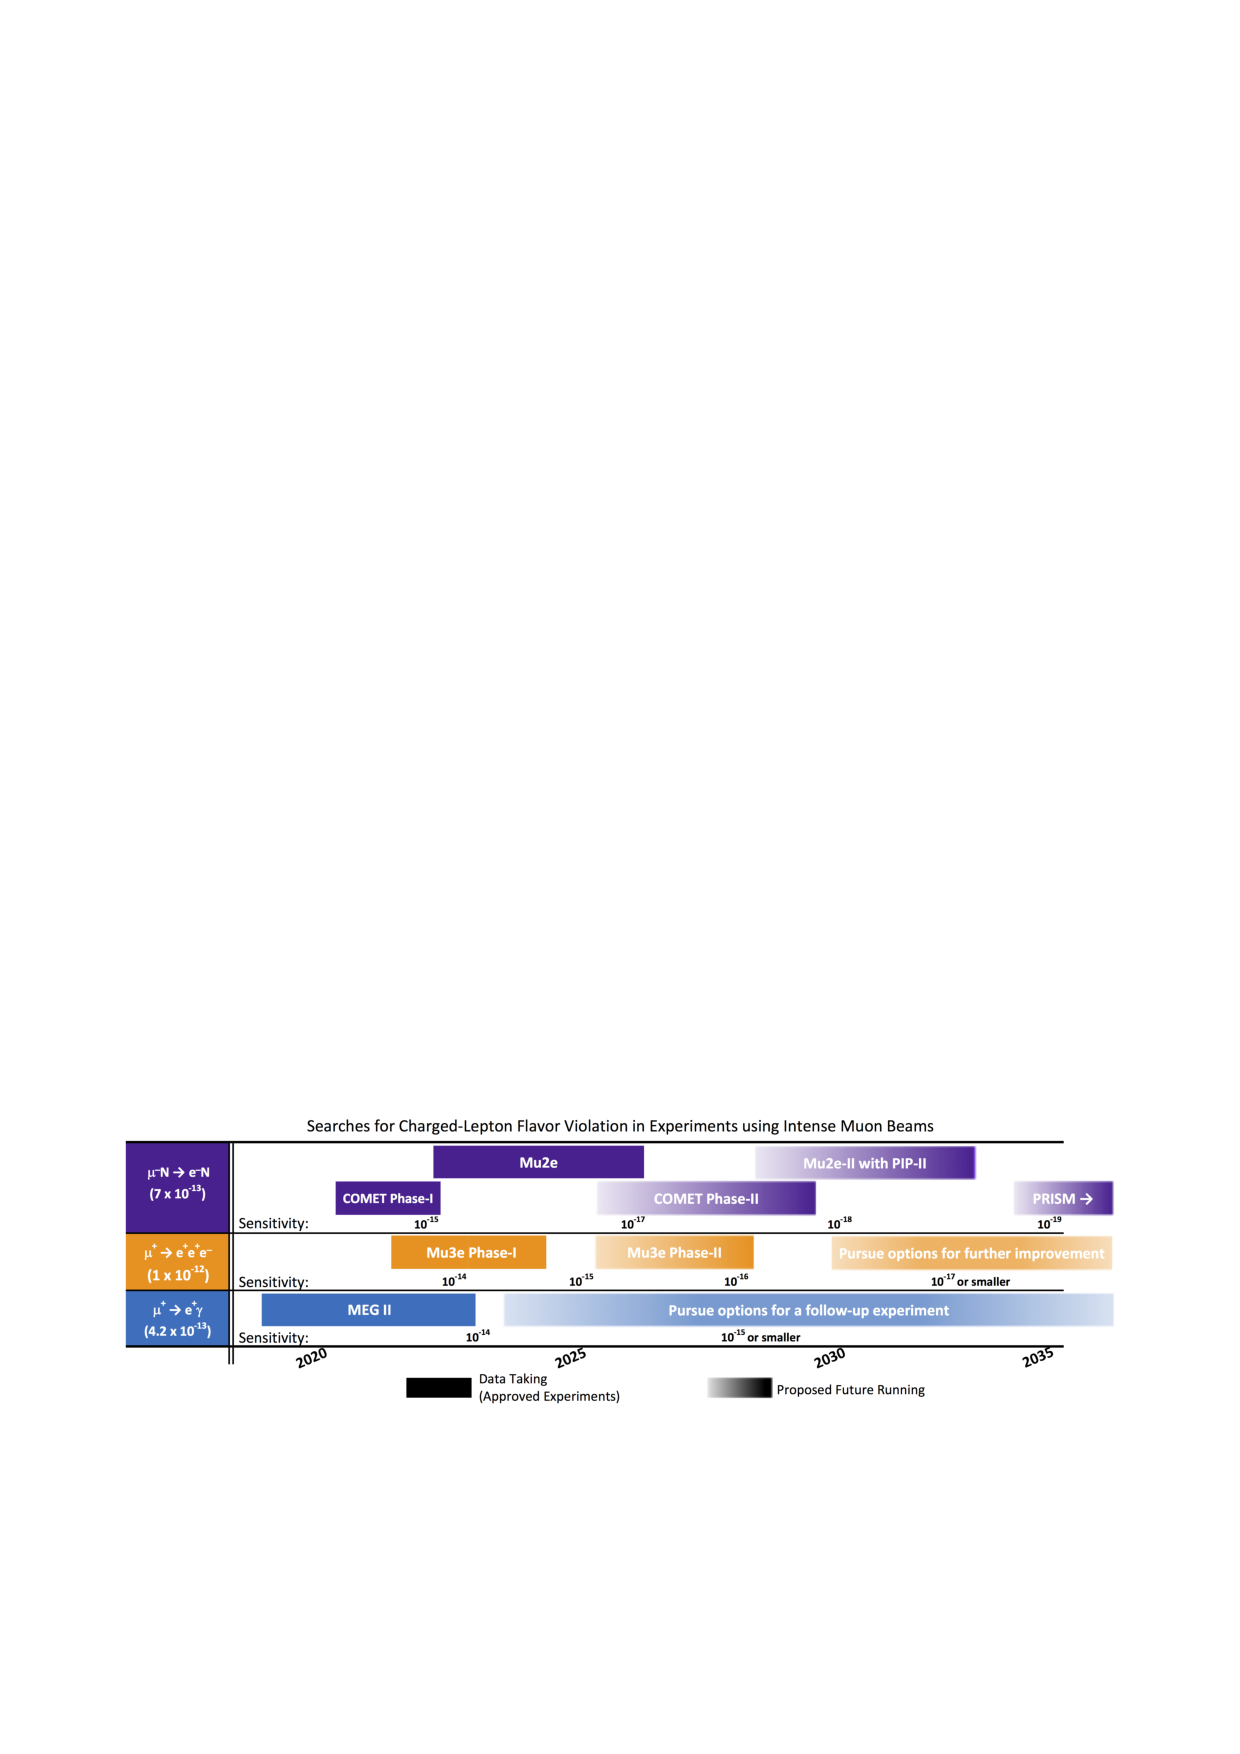
\includegraphics[width=1.0\textwidth]{\main/Flavour/figs/Muon-timeline.pdf} 
\end{center}
\caption{Planned data taking schedules for current experiments searching for LFV muon-electron transitions, as well as the schedules and expected sensitivities for future upgrades~\cite{Baldini:2018uhj}.
  }\label{fig:cLFV:muon:chrono} 
\end{figure}

